\documentclass[11pt,a4paper]{article}

\usepackage[utf8]{inputenc}
\usepackage[T1]{fontenc}
\usepackage[polish]{babel}
\usepackage{amsmath,amssymb,amsfonts}
\usepackage{geometry}
\usepackage{graphicx}
\usepackage{booktabs}
%\usepackage{microtype} % Zakomentowane: w darmowej wersji Overleaf często powoduje timeout
\IfFileExists{float.sty}{\usepackage{float}}{}
\usepackage{xcolor}
\usepackage{hyperref}
% subcaption i listings są w szablonie projektu. Ładują się, gdy są zainstalowane.
\IfFileExists{subcaption.sty}{\usepackage{subcaption}}{}
\IfFileExists{listings.sty}{\usepackage{listings}}{}

\geometry{
    a4paper,
    top=25mm,
    bottom=25mm,
    left=25mm,
    right=25mm
}

\hypersetup{
    colorlinks=true,
    linkcolor=blue!70!black,
    citecolor=blue!70!black,
    urlcolor=blue!70!black,
    pdftitle={Pamiec skojarzeniowa z uzyciem sieci Hopfielda}
}

\graphicspath{{figures/}{experiments/results/}}

\IfFileExists{listings.sty}{%
\lstset{
    basicstyle=\ttfamily\footnotesize,
    breaklines=true,
    frame=single,
    backgroundcolor=\color{gray!5},
    keywordstyle=\color{blue}\bfseries,
    commentstyle=\color{green!50!black}\itshape,
    stringstyle=\color{red!60!black},
    numbers=left,
    numberstyle=\tiny\color{gray},
    stepnumber=1,
    tabsize=4,
    showstringspaces=false,
    language=Python
}}{}

\begin{document}

\begin{titlepage}
    \centering
    {\fontsize{60}{30}\selectfont \textbf{Sieci Neuronowe} \par}
    \vspace{1.5cm}
    {\fontsize{30}{20}\selectfont Projekt 2 \par}
    \vspace{5cm}
    {\fontsize{36}{20}\selectfont \textbf{Pamięć skojarzeniowa z użyciem sieci Hopfielda} \par}
    \vspace{7.5cm}

    {\fontsize{26}{20}\selectfont
    Sandra Adamiec\\
    Yahor Kachanouski
    \par}
    \vspace{0.5cm}
    \vfill

    {\large listopad 2026 \par}

\end{titlepage}

\tableofcontents
\newpage

\section{Wprowadzenie i cele projektu}

\subsection{Wprowadzenie}
Sieć Hopfielda jest rekurencyjną siecią neuronową, która działa jak pamięć skojarzeniowa \cite{hopfield1982}. Służy do przechowywania niewielkiej liczby wzorców binarnych, na przykład czarno-białych rysunków, i do odtworzenia całego wzorca z wejścia uszkodzonego albo niepełnego. Podaje się treść podobną do zapamiętanej. Sieć uzupełnia ją do całego rysunku.

Stan sieci jest wektorem o współrzędnych \(\pm 1\). Jedna współrzędna to jeden neuron. Gdy wzorzec jest obrazem, neuron odpowiada pikselowi, więc bieżący stan rysuje się jako prostokątna bitmapa. Połączenia między neuronami są symetryczne. W każdym kroku neuron przyjmuje znak sumy stanów pozostałych neuronów, ważonej tymi połączeniami. Wzorzec jest zapamiętany, gdy taka operacja zostawia go bez zmiany. Wejście leżące dostatecznie blisko tego stanu schodzi do niego w kolejnych krokach.

Rysunek~\ref{fig:recall_demo} pokazuje to na zbiorze \texttt{large-25x25}. Sieć nauczona regułą Hebba dostaje sześć obrazów \(25\times 25\), czyli \(625\) neuronów. Dom jest wzorcem stabilnym. Po odwróceniu \(20\%\) jego pikseli jeden krok synchroniczny przywraca zapisany rysunek.

\begin{figure}[!htbp]
    \centering
    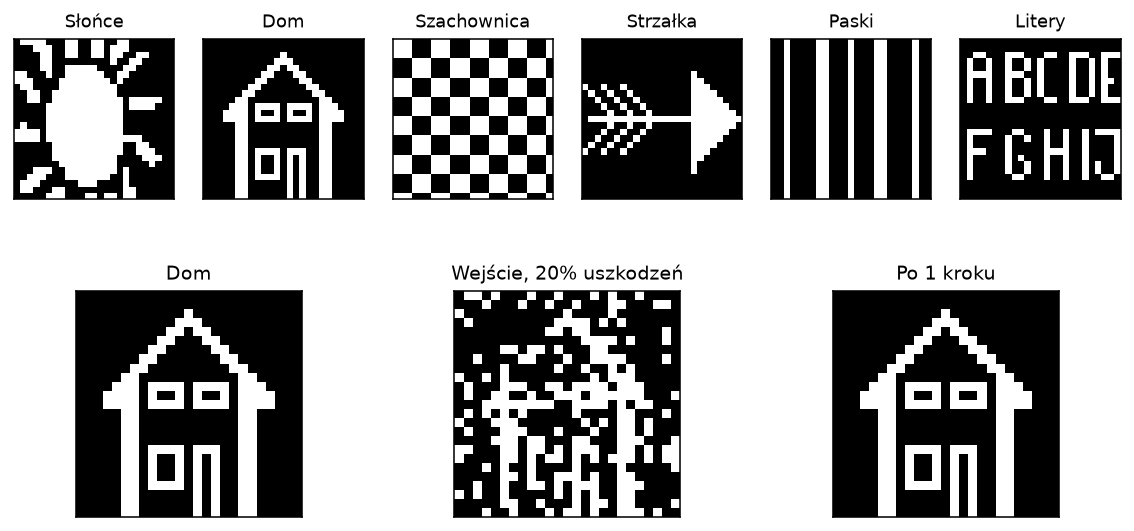
\includegraphics[width=\textwidth]{dzialanie.png}
    \caption{Działanie pamięci na zbiorze \texttt{large-25x25}, uczenie regułą Hebba. Górny rząd: wzorce podane do sieci. Dolny rząd: dom, ten sam rysunek z odwróconymi \(20\%\) pikseli oraz stan po jednym kroku synchronicznym.}
    \label{fig:recall_demo}
\end{figure}

Celem projektu jest samodzielna implementacja tej pamięci oraz sprawdzenie, w jakich warunkach sieć naprawdę zapamiętuje podane wzorce. Wzorce są wpisywane w symetryczną macierz wag, a odtworzenie polega na zejściu stanu do minimum energii. Implementacja obejmuje dwie reguły uczenia, regułę Hebba i regułę Erkkiego Oji, oraz dwa tryby dynamiki: synchroniczny i asynchroniczny.

\subsection{Wymagania i cele zdefiniowane w zadaniu}
Zgodnie ze specyfikacją projektu zrealizowano następujące założenia:
\begin{enumerate}
    \item \textbf{Model i konfiguracja:}
    \begin{itemize}
        \item Sieć o liczbie neuronów równej długości wzorca. Bitmapa \(w \times h\) daje \(N = wh\) neuronów, a macierz wag jest budowana przy uczeniu pod tę długość. Rozmiar prostokąta jest czytany z nazwy pliku, na przykład \texttt{animals-14x9.csv} oznacza 14 kolumn i 9 wierszy.
        \item Wizualizacja bieżącego stanu jako czarno-białej bitmapy oraz podgląd kolejnych kroków aż do stanu stałego, cyklu albo limitu kroków.
        \item Dwa warianty symulacji. W kroku synchronicznym wszystkie neurony liczone są z tego samego stanu. W kroku asynchronicznym neurony są odwiedzane w losowej kolejności i późniejszy neuron widzi już zmiany wcześniejszych.
    \end{itemize}

    \item \textbf{Reguły uczenia:}
    \begin{itemize}
        \item Reguła Hebba, jednorazowy zapis wszystkich wzorców.
        \item Reguła Oji, uczenie przyrostowe z tłumieniem wag (\(\eta = 0{,}01\), \(200\) epok).
    \end{itemize}

    \item \textbf{Wymagany zakres badań:}
    \begin{itemize}
        \item skuteczność obu reguł i liczba stabilnych wzorców uczących,
        \item które z dostarczonych zbiorów sieć zapamiętuje, a które nie, oraz dlaczego część wzorców nie jest stabilna,
        \item różnica odzysku na parach rysunków \(25\times 25\) i \(25\times 50\),
        \item odzysk oryginału z uszkodzonego wejścia w zależności od liczności i rodzaju zbioru,
        \item porównanie zbioru podobnych wzorców ze zbiorem zróżnicowanym o tej samej liczności,
        \item reakcja na losowe wejście,
        \item możliwie liczny zbiór wektorów o długości 25, w którym każdy wzorzec jest stabilny,
        \item zbiór uczący i wejście prowadzące do oscylacji między dwoma stanami,
        \item eksperyment na bitmapach co najmniej \(200\times 300\), na zdjęciach kotów spoza materiałów projektu.
    \end{itemize}
\end{enumerate}

\section{Architektura i implementacja sieci}

\subsection{Stan, wagi i moduły}
Stan sieci jest wektorem \(s \in \{-1,1\}^N\). Jedna współrzędna to jeden neuron i, przy obrazie, jeden piksel. Nie da się ustawić liczby neuronów niezależnie od długości wzorca: wzorzec o 126 pikselach wchodzi tylko do sieci o 126 neuronach. Konfiguracja polega na podaniu innego zbioru. Klasa \texttt{HopfieldNetwork} buduje wtedy macierz \(N \times N\).

Kod jest podzielony na trzy warstwy:
\begin{itemize}
    \item \texttt{hopfield.py}: uczenie Hebba i Oji, krok synchroniczny, krok asynchroniczny, energia, test stabilności oraz metoda \texttt{evolve}, która zapisuje trajektorię i rozróżnia stan stały, cykl oraz wyczerpanie limitu kroków.
    \item \texttt{visualization.py}: rysowanie jednego stanu, całego zbioru i kolejnych kadrów zbiegania. Szerokie obrazki są łamane na wiersze, żeby cały zbiór mieścił się w oknie.
    \item \texttt{experiments/}: osobny skrypt na każdy punkt zadania. Wydruk jest od razu zapisywany do \texttt{experiments/results}.
\end{itemize}
Operacje na wagach i polach są zwektoryzowane w \texttt{numpy}. Krok synchroniczny to jeden iloczyn macierz--wektor, bez pętli po neuronach.

\subsection{Reguła Hebba i powód, dla którego pamięta}
Stan neuronu \(i\) jest bitem \(s_i \in \{-1, 1\}\). W reprezentacji obrazu wartość \(+1\) odpowiada pikselowi białemu, a wartość \(-1\) pikselowi czarnemu. Waga \(w_{ij} = w_{ji}\) opisuje połączenie neuronów \(i\) oraz \(j\): wartość dodatnia sprzyja zgodności ich znaków, wartość ujemna sprzyja znakom przeciwnym. Pole lokalne neuronu \(i\) jest ważoną sumą stanów pozostałych neuronów,
\[
    h_i = \sum_{j \neq i} w_{ij}\, s_j.
\]
Aktualizacja przyjmuje \(s_i \leftarrow \operatorname{sgn}(h_i)\). Przy polu zerowym stan neuronu pozostaje bez zmiany.

Reguła Hebba utrwala współaktywność neuronów \cite{hebb1949}. Dla pary współrzędnych wzorca \(x\) iloczyn \(x_i x_j\) wynosi \(+1\) przy zgodnych znakach oraz \(-1\) przy znakach przeciwnych. Wkłady \(P\) wzorców są sumowane i skalowane przez \(1/N\),
\[
    w_{ij} = \frac{1}{N}\sum_{\mu=1}^{P} x_i^{\mu} x_j^{\mu}, \qquad i \neq j.
\]
Przekątna jest zerowana, ponieważ neuron nie jest sprzężony sam ze sobą. Człon diagonalny miałby wartość \(P/N\) niezależnie od stanu i nie różnicowałby wzorców. Macierz wag ma postać
\begin{equation}
\label{eq:hebb}
    W = \frac{1}{N}\sum_{\mu=1}^{P} x^{\mu}(x^{\mu})^{\top}, \qquad w_{ii} = 0.
\end{equation}
Macierz \(x(x)^{\top}\) zawiera iloczyny \(x_i x_j\) jednego wzorca. Zapis odbywa się jednorazowo, bez epok i bez współczynnika uczenia.

Czynnik \(1/N\) jest normalizacją tej sumy, a nie współczynnikiem uczenia. Bez niego wkład własnego wzorca do pola byłby rzędu \(N\), bo \(x^{\nu}\cdot x^{\nu} = N\). Po podzieleniu przez liczbę neuronów sygnał w~\eqref{eq:field} jest rzędu \(1\) i nie rośnie razem z rozmiarem bitmapy. Atraktorów to nie zmienia: dynamika używa znaku pola, a pomnożenie całej macierzy \(W\) przez dowolną stałą dodatnią ten znak zachowuje.

Mechanizm ilustruje sieć o trzech neuronach i wzorzec \(x = (1, 1, -1)\). Dwie pierwsze współrzędne mają zgodny znak, trzecia ma znak przeciwny. Przy \(N = 3\)
\[
    w_{12} = \tfrac13, \qquad w_{13} = -\tfrac13, \qquad w_{23} = -\tfrac13.
\]
Pole na wzorcu \(s = (1, 1, -1)\) liczone jest osobno dla każdego neuronu, z pominięciem jego własnej wagi:
\begin{align*}
    h_1 &= w_{12}s_2 + w_{13}s_3 = \tfrac13\cdot 1 + \bigl(-\tfrac13\bigr)\cdot(-1) = \tfrac23, \\
    h_2 &= w_{21}s_1 + w_{23}s_3 = \tfrac13\cdot 1 + \bigl(-\tfrac13\bigr)\cdot(-1) = \tfrac23, \\
    h_3 &= w_{31}s_1 + w_{32}s_2 = \bigl(-\tfrac13\bigr)\cdot 1 + \bigl(-\tfrac13\bigr)\cdot 1 = -\tfrac23.
\end{align*}
Zatem \(h = (2/3,\ 2/3,\ -2/3)\). Znaki pola są zgodne ze wzorcem, więc stan jest stabilny. Po odwróceniu trzeciej współrzędnej stan wynosi \((1, 1, 1)\) i
\[
    h_3 = w_{31}s_1 + w_{32}s_2 = \bigl(-\tfrac13\bigr)\cdot 1 + \bigl(-\tfrac13\bigr)\cdot 1 = -\tfrac23.
\]
Aktualizacja przywraca bit \(-1\). Ujemne wagi \(w_{13}\) i \(w_{23}\) wymuszają znak trzeciego neuronu przeciwny do dwóch pierwszych.

Dla \(P > 1\) do pola dochodzi wkład pozostałych wzorców. Podstawienie wzorca uczącego \(x^{\nu}\) daje
\begin{align}
    h_i(x^{\nu})
    &= \sum_{j \neq i} w_{ij} x_j^{\nu}
    = \frac{1}{N}\sum_{\mu=1}^{P} x_i^{\mu}\bigl(x^{\mu}\cdot x^{\nu} - x_i^{\mu} x_i^{\nu}\bigr) \nonumber \\
    &= \Bigl(1 - \frac{P}{N}\Bigr) x_i^{\nu}
     + \frac{1}{N}\sum_{\mu \neq \nu} (x^{\mu}\cdot x^{\nu})\, x_i^{\mu}.
    \label{eq:field}
\end{align}
Człon \(x_i^{\mu} x_i^{\nu}\) wynika z zerowej przekątnej: iloczyn skalarny zawiera współrzędną \(i\), a suma definiująca pole jej nie zawiera. Dla \(\mu = \nu\) zachodzi \(x^{\nu}\cdot x^{\nu} = N\) oraz \((x_i^{\nu})^2 = 1\), więc wkład własnego wzorca wynosi \((1 - 1/N)\, x_i^{\nu}\). Wkłady \(\mu \neq \nu\) dokładają z tej samej przekątnej łącznie \(-(P-1)/N\, x_i^{\nu}\). Stąd czynnik \(1 - P/N\).

Pierwszy składnik~\eqref{eq:field} jest sygnałem. Ma znak współrzędnej wzorca i moduł bliski jedności przy \(P \ll N\). Drugi składnik jest przesłuchem: wzorzec \(\mu\) wnosi w neuronie \(i\) bit \(x_i^{\mu}\) z wagą proporcjonalną do podobieństwa \(x^{\mu}\cdot x^{\nu}\). Wzorzec jest stabilny, gdy \(h_i x_i^{\nu} \ge 0\) dla każdego \(i\). Aktualizacja nie zmienia wtedy żadnego bitu.

Dla wzorców losowych przesłuch ma średnią zero. Typowy wzorzec pozostaje atraktorem do obciążenia
\begin{equation}
    P_{\max} \approx 0{,}14\, N,
\end{equation}
czyli \(\alpha = P/N \approx 0{,}14\) \cite{amit1985,amit1987}. McEliece i współpracownicy podają ostrzejszy rząd \(N/(2\ln N)\) na stabilność wszystkich losowych wzorców jednocześnie \cite{mceliece1987}. Wzorce o wspólnych krawędziach osiągają iloczyny rzędu \(N\), a nie \(\sqrt{N}\), więc tracą stabilność przy znacznie mniejszym \(\alpha\).

Przy wagach symetrycznych i zerowej przekątnej energia
\begin{equation}
\label{eq:energy}
    E(s) = -\frac12 s^{\top} W s
\end{equation}
nie rośnie, jeżeli aktualizowany jest jeden neuron \cite{hopfield1982}. Zamiana bitu \(s_k\) na \(s_k' = -s_k\) zmienia energię o \(\Delta E = -2 s_k' h_k\). Reguła znaku przyjmuje \(s_k' = \operatorname{sgn}(h_k)\), więc \(\Delta E = -2|h_k| < 0\), o ile pole jest niezerowe. Dynamika asynchroniczna schodzi do minimum lokalnego. Zapamiętany wzorzec jest takim minimum, gdy przesłuch w~\eqref{eq:field} nie zmienia znaku sygnału. Stan początkowy z basenu tego minimum zbiega do wzorca.

Jeżeli stan \(s\) jest stabilny i wszystkie pola są niezerowe, stabilny jest także \(-s\), ponieważ zmiana znaku stanu zmienia znak pola. Negacja wzorca jest więc dodatkowym atraktorem, niewystępującym w zbiorze uczącym. Oprócz niej powstają stany pozorne. Mieszanka kilku wzorców ma w każdej współrzędnej znak sumy tych wzorców \cite{amit1985}: współrzędne wspólne otrzymują w \(W\) kilka zgodnych składników, a współrzędne różniące się redukują się wzajemnie.

\subsection{Reguła Oji i powód, dla którego ogranicza wagi}
Jednokrotne zastosowanie reguły Hebba wyznacza macierz~\eqref{eq:hebb}. Wielokrotne dodawanie tego samego iloczynu \(x_i x_j\) zwiększałoby wagi proporcjonalnie do liczby prezentacji, przy zachowanym znaku pola. Reguła Erkkiego Oji uzupełnia krok Hebba członem tłumiącym, który ogranicza wzrost wag \cite{oja1982}.

W zaimplementowanej procedurze wagi startują od zera. Wzorce są prezentowane kolejno przez zadaną liczbę epok. Po każdej prezentacji, dla \(i \neq j\),
\begin{equation}
\label{eq:oja}
    \Delta w_{ij} = \eta\,(x_i x_j - w_{ij}).
\end{equation}
Składnik \(\eta\, x_i x_j\) jest krokiem Hebba o wielkości \(\eta\): zgodne znaki zwiększają wagę, znaki przeciwne ją zmniejszają. Składnik \(-\eta\, w_{ij}\) sprowadza wagę ku zeru. W pomiarach przyjęto \(\eta = 0{,}01\) oraz \(200\) epok. Po każdym wzorcu przekątna jest zerowana.

Równanie~\eqref{eq:oja} przyciąga \(w_{ij}\) do iloczynu \(x_i x_j \in \{+1, -1\}\) bieżącego wzorca. Przy jednym wzorcu, \(\eta = 0{,}5\) i starcie od zera kolejne wartości wagi zgodnej pary wynoszą \(0\), \(0{,}5\), \(0{,}75\), \(0{,}875\) i zbiegają do \(1\). Reguła Hebba dla tego samego wzorca wyznacza od razu \(w_{ij} = 1/N\). Obie wartości są dodatnie, więc znak pola jest zgodny.

Przy wielu wzorcach kolejne prezentacje wskazują dla tej samej pary przeciwne iloczyny. Po dużej liczbie epok i przy małym \(\eta\) wagi zbiegają do średniej tych iloczynów,
\[
    W^{\mathrm{Oja}} \approx \frac{1}{P}\sum_{\mu=1}^{P} x^{\mu}(x^{\mu})^{\top}.
\]
Macierz Hebba jest tą samą sumą podzieloną przez \(N\), zatem
\[
    W^{\mathrm{Oja}} \approx \frac{N}{P}\, W^{\mathrm{Hebb}}.
\]
Czynnik \(N/P\) jest dodatni. Znak pola \(Ws\) nie zależy od dodatniego skalowania macierzy, więc w granicy obu reguł atraktory są wspólne.

Reguła~\eqref{eq:oja} jest szczególnym przypadkiem reguły podanej przez Oję dla neuronu liniowego o wyjściu \(y = w \cdot x\),
\[
    \Delta w = \eta\, y\,(x - y w).
\]
Składnik \(yx\) odpowiada krokowi Hebba, a składnik \(-y^2 w\) ogranicza normę wektora wag. Przy odpowiednich danych neuron uczy się pierwszego kierunku głównego \cite{oja1982}. W pamięci autoasocjacyjnej wyjście neuronu \(i\) podczas uczenia jest ustalone na bit wzorca, \(y_i = x_i\). Dla bitów \(\pm 1\) zachodzi \(y_i^2 = 1\), więc
\[
    \Delta w_{ij}
    = \eta\, x_i (x_j - x_i w_{ij})
    = \eta\,(x_i x_j - w_{ij}),
\]
zgodnie z~\eqref{eq:oja}. Implementacja stosuje bezpośrednio tę postać.

Różnice obserwowane w eksperymentach wynikają ze skończonej liczby \(200\) epok oraz z zerowania przekątnej po każdym wzorcu. Przy wzorcu o małym marginesie \(h_i x_i\) zmiana ta może odwrócić jeden bit. Po zbieżności obie reguły wyznaczają ten sam kierunek pola, więc reguła Oji nie zwiększa pojemności względem reguły Hebba.

\subsection{Dwa tryby dynamiki}
Nowy stan neuronu wyznacza znak pola. Przy \(h_i = 0\) bit zostaje bez zmiany. W kroku synchronicznym wszystkie pola liczone są ze starego stanu, więc energia~\eqref{eq:energy} nie musi spadać i możliwy jest cykl o okresie dwa. W kroku asynchronicznym zmiana jednego neuronu energię obniża, więc przebieg kończy się w stanie stałym. Metoda \texttt{evolve} zapisuje kolejne kadry i zwraca status \texttt{stable}, \texttt{cycle} albo \texttt{max\_steps}.

Dla bitmap o \(N = 60\,000\) macierz wag nie mieści się w pamięci. Pole Hebba da się policzyć wprost ze wzorców. Dla macierzy \(X \in \{-1,1\}^{P \times N}\) i stanu \(s\)
\begin{equation}
\label{eq:implicit}
    h = \frac{1}{N} X^{\top}(Xs) - \frac{P}{N}s.
\end{equation}
To jest wzór~\eqref{eq:hebb} z wyzerowaną przekątną. Iloczyn \(Xs\) ma tylko \(P\) liczb.

\section{Eksperyment 1: Skuteczność reguł i stabilność wzorców}
\label{sec:exp_stability}

\subsection{Opis eksperymentu}
Celem pierwszego eksperymentu było porównanie obu reguł uczenia oraz ustalenie, które z dostarczonych zbiorów sieć zapamiętuje. Wzorzec uznano za nauczony, gdy jeden krok synchroniczny zostawia go bez zmiany. To jest dokładnie warunek \(h_i x_i \ge 0\) dla wszystkich neuronów.

Dla każdego pliku z katalogu \texttt{datasets} nauczono dwie niezależne sieci. Reguła Oji używała \(\eta = 0{,}01\) i \(200\) epok. Zbiory obejmują małe ikony \(7\times 7\), zwierzęta \(14\times 9\), litery, znaki OCRA oraz dwie wersje dużych rysunków. Żaden zbiór nie przekracza granicy \(0{,}14N\) liczonej tak, jak dla wzorców losowych. Tabela~\ref{tab:stable} podaje obciążenie \(\alpha = P/N\) i liczbę stabilnych wzorców. Udział stabilnych wzorców jest na rysunku~\ref{fig:stability}.

\begin{table}[!htbp]
\centering
\caption{Liczba stabilnych wzorców uczących po regule Hebba i po regule Oji.}
\label{tab:stable}
\begin{tabular}{lrrrr}
\toprule
Zbiór & \(P\) & \(N\) & Hebb & Oja \\
\midrule
\texttt{small-7x7}        &  5 &   49 &  3/5  &  3/5  \\
\texttt{animals-14x9}     &  6 &  126 &  2/6  &  2/6  \\
\texttt{letters-abc-8x12} &  3 &   96 &  0/3  &  0/3  \\
\texttt{letters-14x20}    & 26 &  280 &  0/26 &  0/26 \\
\texttt{OCRA-12x30-cut}   &  7 &  360 &  1/7  &  0/7  \\
\texttt{large-25x25}      &  6 &  625 &  5/6  &  5/6  \\
\texttt{large-25x25.plus} & 15 &  625 &  1/15 &  1/15 \\
\texttt{large-25x50}      &  6 & 1250 &  0/6  &  0/6  \\
\bottomrule
\end{tabular}
\end{table}

\begin{figure}[!htbp]
    \centering
    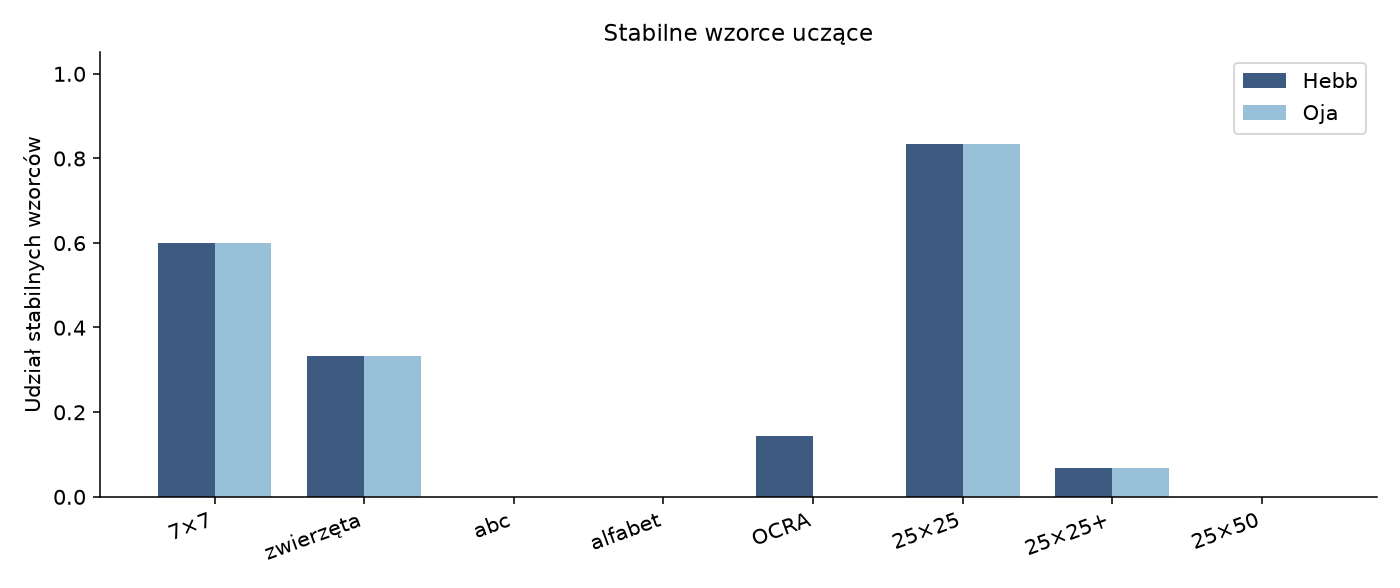
\includegraphics[width=\textwidth]{stabilnosc.png}
    \caption{Udział wzorców uczących, które pozostają stanami stabilnymi. Słupki Hebba i Oji pokrywają się poza zbiorem OCRA.}
    \label{fig:stability}
\end{figure}

\subsection{Opis wyników i dyskusja}
\begin{enumerate}
    \item \textbf{Reguły dają tę samą pamięć.}
    Liczby stabilnych wzorców są identyczne dla Hebba i Oji na siedmiu z ośmiu zbiorów. To jest konsekwencja skali: po zbieżności \(W^{\mathrm{Oja}}\) jest dodatnią wielokrotnością macierzy Hebba, a znak pola od skali nie zależy. Jedyna różnica dotyczy OCRA, gdzie Hebb utrwala 1 wzorzec z 7, a Oja żadnego. Margines \(h_i x_i\) tego wzorca jest na tyle mały, że skończone uczenie Oji i zerowanie przekątnej wewnątrz pętli przewraca jeden bit. Reguła Oji nie zwiększa pojemności względem Hebba.

    \item \textbf{Granica \(0{,}14N\) nie wystarcza do przewidzenia wyniku.}
    Najlepiej wypada \texttt{large-25x25}: 5 z 6 wzorców przy \(\alpha = 0{,}010\). Pary rysunków zgadzają się w 49--73\% pikseli. Wypada tylko strzałka. Ten sam rozmiar z piętnastoma wzorcami (\texttt{large-25x25.plus}) zostawia już 1 wzorzec z 15, choć \(\alpha = 0{,}024\) nadal leży daleko poniżej \(0{,}14\). Dodatkowe rysunki powiększają sumę przesłuchu w~\eqref{eq:field}.

    \item \textbf{Korelacja psuje zbiory o małym obciążeniu.}
    Trzy litery \(8\times 12\) mają \(\alpha = 0{,}031\), a zgadzają się w 89--92\% pikseli. Nie jest stabilna żadna. Alfabet \(14\times 20\) (26 liter, zgodność 74--99\%) też nie utrwala ani jednego znaku. Znaki OCRA, o wspólnym szkielecie i zgodności 53--74\%, zostawiają co najwyżej jeden wzorzec. Iloczyn \(x^{\mu}\cdot x^{\nu}\) jest wtedy rzędu \(N\), więc drugi składnik~\eqref{eq:field} przebija sygnał. To jest zgodne z zastrzeżeniem Amita, Gutfreunda i Sompolinsky'ego oraz McEliece'a: granica \(0{,}14N\) dotyczy wzorców losowych \cite{amit1985,mceliece1987}.

    \item \textbf{Zwierzęta tworzą mieszankę.}
    Zbiór \(14\times 9\) ma sześć wzorców, \(\alpha = 0{,}048\) i zgodność par 54--69\%. Stabilne zostają tylko dwa. Wzorce 1, 2, 3 i 6 schodzą do jednego stanu, który jest znakiem sumy \(x^{1}+x^{2}+x^{3}+x^{6}\). To jest stan pozorny opisany w \cite{amit1985}: piksele wspólne dla kilku zwierząt dostają w \(W\) kilka głosów, a piksele różniące kasują się nawzajem. Mieszanka jest głębszym minimum niż osobne rysunki, więc dynamika ją wybiera.

    \item \textbf{Mały zbiór \(7\times 7\) leży przy obu ograniczeniach naraz.}
    Tutaj \(\alpha = 0{,}102\), blisko granicy losowej, a zgodność par sięga 76\%. Stabilne są 3 wzorce z 5. Ani sama liczność, ani sama korelacja nie tłumaczy wyniku. Obie wchodzą do~\eqref{eq:field}.
\end{enumerate}

\section{Eksperyment 2: Odzysk z uszkodzonego wejścia}
\label{sec:exp_recall}

\subsection{Opis eksperymentu}
Celem drugiego eksperymentu było zmierzenie, jak często uszkodzony wzorzec wraca dokładnie do oryginału, oraz od czego ta częstość zależy.

Dla każdego wzorca odwracano 10\%, 20\% i 30\% bitów. Liczba odwróceń to część całkowita z \(N\) razy poziom szumu. Sieć puszczano synchronicznie, najwyżej przez 20 kroków. Sukcesem była dokładna zgodność stanu końcowego z oryginałem, a nie samo podobieństwo. Na każdy wzorzec przypadało 10 niezależnych uszkodzeń. Osobno liczono sukces wśród wszystkich wzorców i tylko wśród tych, które są stabilne. Jeżeli zbiór nie ma stabilnych wzorców, odzysk oryginału jest niemożliwy: dynamika nie może stanąć w punkcie, który punktem stałym nie jest.

Pomiary powtórzono dla Hebba i Oji. Tabela~\ref{tab:recall} podaje regułę Hebba. Liczba po ukośniku dotyczy samych wzorców stabilnych. Kreska oznacza, że takich wzorców nie ma. Mapa odzysku na całych zbiorach jest na rysunku~\ref{fig:recall}.

\begin{table}[!htbp]
\centering
\caption{Procent dokładnych odzyskań, reguła Hebba, 10 prób na wzorzec. Zapis \(a/b\): wszystkie wzorce / tylko stabilne.}
\label{tab:recall}
\begin{tabular}{lrrr}
\toprule
Zbiór & 10\% & 20\% & 30\% \\
\midrule
\texttt{small-7x7}        & 42/70 & 46/77 & 32/53 \\
\texttt{animals-14x9}     & 27/80 & 20/60 & 22/65 \\
\texttt{letters-abc-8x12} &  0/-- &  0/-- &  0/-- \\
\texttt{letters-14x20}    &  0/-- &  0/-- &  0/-- \\
\texttt{OCRA-12x30-cut}   &  7/50 &  7/50 &  4/30 \\
\texttt{large-25x25}      & 72/86 & 65/78 & 63/76 \\
\texttt{large-25x25.plus} & 7/100 & 7/100 & 7/100 \\
\texttt{large-25x50}      &  0/-- &  0/-- &  0/-- \\
\bottomrule
\end{tabular}
\end{table}

\begin{figure}[!htbp]
    \centering
    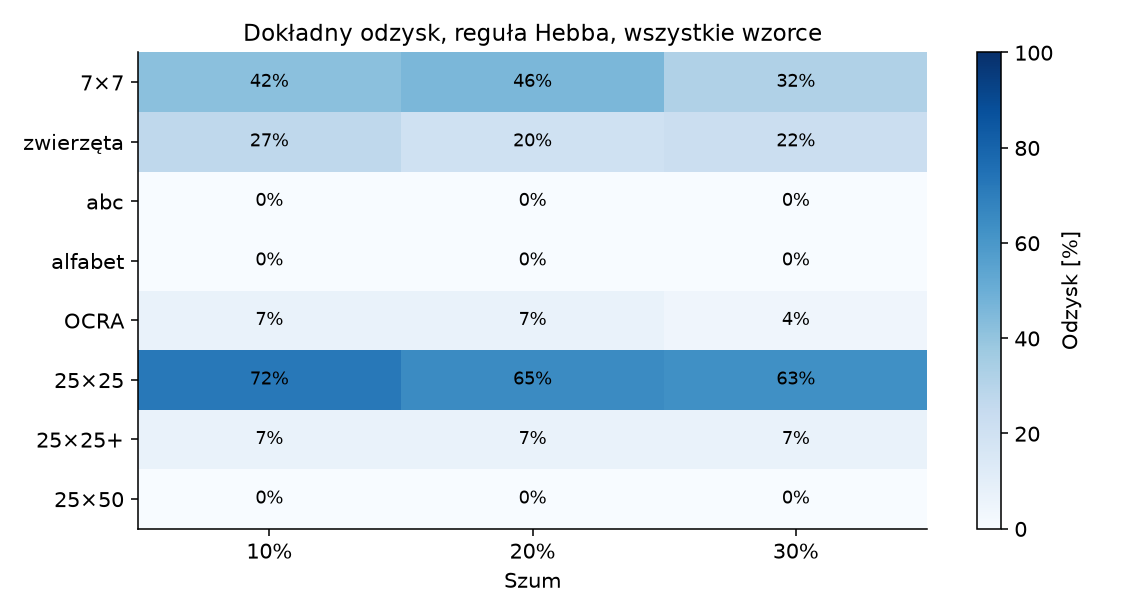
\includegraphics[width=0.92\textwidth]{odzysk.png}
    \caption{Dokładny odzysk oryginału przy regule Hebba, liczony na wszystkich wzorcach zbioru. Zera odpowiadają zbiorom bez stabilnych wzorców uczących.}
    \label{fig:recall}
\end{figure}

\subsection{Opis wyników i dyskusja}
\begin{enumerate}
    \item \textbf{Odzysk idzie za stabilnością.}
    Litery, alfabet i zbiór \(25\times 50\) mają 0\% na każdym poziomie szumu. Oryginał nie jest atraktorem, więc żadne uszkodzenie, także bardzo małe, nie może do niego wrócić. W \texttt{large-25x25.plus} jedyny stabilny wzorzec wraca w 100\% prób nawet przy 30\% szumu, ale stanowi jedną piętnastą zbioru, stąd 7\% na całość.

    \item \textbf{Basen stabilnego wzorca jest ograniczony.}
    Na \(7\times 7\) odzysk wśród stabilnych spada z 70\% przy 10\% szumu do 53\% przy 30\%. Na \(25\times 25\) spadek jest łagodniejszy: 86\%, 78\% i 76\%. Większa sieć i słabsza korelacja zostawiają szerszy basen, co jest zgodne z tym, że przesłuch w~\eqref{eq:field} maleje wraz z \(N\), gdy iloczyny nie rosną proporcjonalnie do \(N\).

    \item \textbf{Sama liczność \(P\) wyniku nie porządkuje.}
    Sześć zwierząt odzyskuje się gorzej niż sześć różnych obrazów \(25\times 25\) (około 20--27\% wobec 63--72\%). Piętnaście obrazów tego samego rozmiaru odzyskuje się prawie wcale. Liczy się, ile wzorców w ogóle zostało atraktorami i jak szeroki jest ich basen. Rodzaj zbioru wchodzi do obu tych liczb przez korelacje.

    \item \textbf{Oja nie zmienia obrazu.}
    Różnice wobec Hebba wynoszą kilka punktów procentowych i mieszczą się w wahaniu dziesięciu losowych masek. Wyjątkiem jest OCRA: brak stabilnego wzorca po Oji zeruje odzysk. To jest ten sam fakt co w tabeli~\ref{tab:stable}, a nie osobny efekt szumu.
\end{enumerate}

\section{Eksperyment 3: Zbiory \(25\times 25\) i \(25\times 50\)}
\label{sec:exp_size}

\subsection{Opis eksperymentu}
W materiałach są dwa zbiory prawie tych samych rysunków, jeden w wersji \(25\times 25\) i drugi w wersji \(25\times 50\). Celem było wyjaśnienie, dlaczego odzysk na nich różni się wyraźnie.

Zastosowano ten sam protokół co w sekcji~\ref{sec:exp_recall}: 10 prób na wzorzec, szum 10\%, 20\% i 30\%, obie reguły, dynamika synchroniczna. Jest to osobny przebieg, więc procenty mogą różnić się o kilka punktów od tabeli~\ref{tab:recall}. Wniosek od tego nie zależy. Wyniki Hebba i Oji są na rysunku~\ref{fig:size}.

\begin{figure}[!htbp]
    \centering
    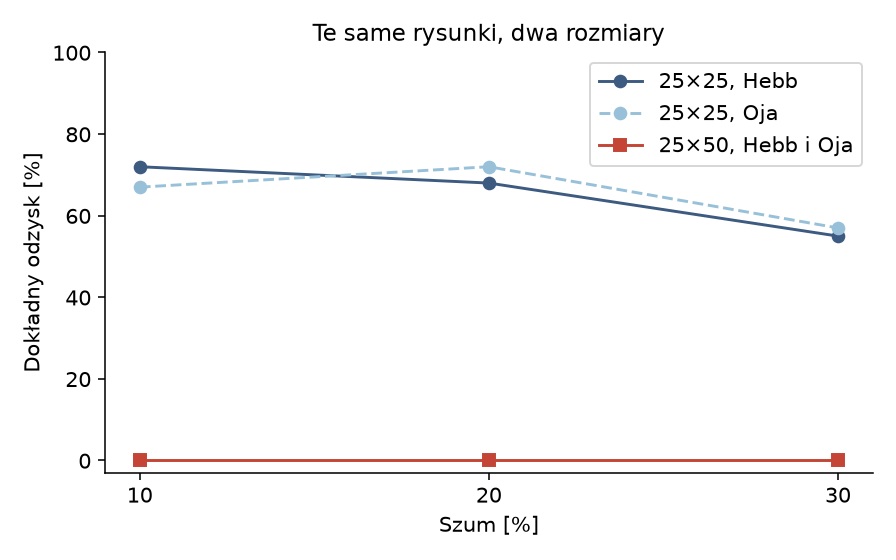
\includegraphics[width=0.78\textwidth]{rozmiar_25.png}
    \caption{Dokładny odzysk tych samych sześciu rysunków na bitmapie \(25\times 25\) i po rozciągnięciu do \(25\times 50\). Krzywe Hebba i Oji dla \(25\times 50\) leżą na zerze.}
    \label{fig:size}
\end{figure}

\subsection{Opis wyników i dyskusja}
\begin{enumerate}
    \item \textbf{Mniejsza bitmapa pamięta, większa nie.}
    Na \(25\times 25\) stabilnych jest 5 wzorców z 6. Odzysk Hebba w tym przebiegu wynosi 72\%, 68\% i 55\%. Na \(25\times 50\) stabilny nie jest żaden z sześciu wzorców, a odzysk wynosi 0\% przy obu regułach i każdym szumie. Średnie podobieństwo stanu końcowego do oryginału zostaje jednak wysokie, około 87--88\%. Sieć nie gubi rysunku. Schodzi do stanu leżącego obok niego.

    \item \textbf{Większe \(N\) powinno pomagać, a nie pomaga.}
    Zbiór \(25\times 50\) ma dwa razy więcej neuronów i dwa razy mniejsze obciążenie (\(0{,}005\) wobec \(0{,}010\)). Dla wzorców losowych byłby łatwiejszy, bo sygnał w~\eqref{eq:field} zostaje rzędu \(1\), a każdy obcy wzorzec jest dzielony przez większe \(N\). Pomiar idzie w przeciwną stronę, więc przyczyną nie jest pojemność liczona wzorem \(0{,}14N\).

    \item \textbf{Rozciągnięcie podnosi korelację.}
    Pary wzorców \(25\times 25\) zgadzają się w 49--73\% pikseli. Po rozciągnięciu do \(25\times 50\) zgodność wynosi 74--87\%. Dodatkowe piksele powielają te same krawędzie, więc iloczyny \(x^{\mu}\cdot x^{\nu}\) rosną prawie razem z \(N\) i nie są tłumione przez mianownik we wzorze na przesłuch. Przesłuch zmienia znak pola we wszystkich sześciu rysunkach. To jest ten sam mechanizm, który zeruje pamięć alfabetu \cite{amit1985,mceliece1987}.
\end{enumerate}

\section{Eksperyment 4: Zbiór podobny i zbiór zróżnicowany}
\label{sec:exp_similarity}

\subsection{Opis eksperymentu}
Zadanie każe porównać zbiór o elementach dość podobnych ze zbiorem zróżnicowanym, przy zbliżonej liczności. Oba zbiory pochodzą z pliku \texttt{large-25x25.plus} i mają te same parametry \(P = 6\), \(N = 625\) oraz \(\alpha = 6/625 \approx 0{,}010\). Z piętnastu wzorców przejrzano wszystkie \(\binom{15}{6} = 5005\) szóstek. Zostawiono szóstkę o największej średniej zgodności par oraz szóstkę o najmniejszej.
\begin{itemize}
    \item \textbf{Podobne}, wzorce 2, 4, 6, 7, 9 i 13: dom, strzałka, litery, helikopter, dinozaur i znak ostrzegawczy. Średnia zgodność par wynosi \(68{,}9\%\), mediana \(69{,}4\%\), zakres \(61{,}3\)--\(74{,}9\%\). Są to rysunki z niedużą ilością bieli na wspólnym czarnym tle.
    \item \textbf{Zróżnicowane}, wzorce 1, 3, 5, 8, 10 i 14: słońce, szachownica, paski, zamek, zagnieżdżone kwadraty i krzyż. Średnia zgodność wynosi \(51{,}2\%\), mediana \(50{,}7\%\), zakres \(36{,}6\)--\(60{,}5\%\).
\end{itemize}
Zakresy zgodności tych dwóch szóstek są rozłączne. Protokół odzysku jest taki sam jak w sekcji~\ref{sec:exp_recall}: szum \(10\%\), \(20\%\) i \(30\%\), \(10\) prób na wzorzec, obie reguły, dynamika synchroniczna. Wyniki Hebba są na rysunku~\ref{fig:similarity}. Reguła Oji dała te same ułamki.

\begin{figure}[!htbp]
    \centering
    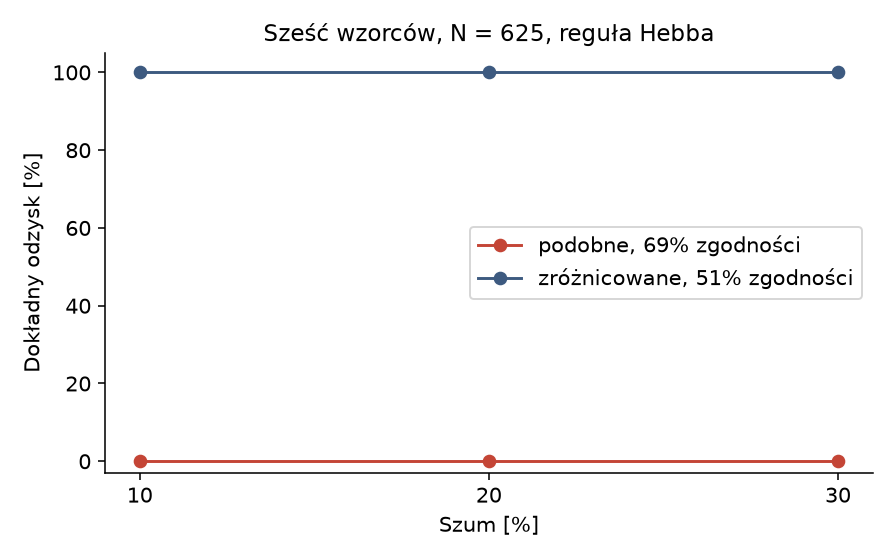
\includegraphics[width=0.78\textwidth]{podobne_zroznicowane.png}
    \caption{Dokładny odzysk przy \(P = 6\) i \(N = 625\). Szóstka o średniej zgodności \(69\%\) nie wraca do oryginału. Szóstka o średniej zgodności \(51\%\) wraca w każdej próbie. Reguła Oji daje ten sam wykres.}
    \label{fig:similarity}
\end{figure}

\subsection{Opis wyników i dyskusja}
\begin{enumerate}
    \item \textbf{Ta sama liczność i ta sama sieć, inna liczba atraktorów.}
    Po Hebba i po Oji szóstka podobna nie utrwala żadnego wzorca, a szóstka zróżnicowana utrwala wszystkie sześć. Odzysk oryginału wynosi odpowiednio \(0\%\) i \(100\%\) przy każdym z trzech poziomów szumu. W zbiorze zróżnicowanym odzysk wśród wzorców stabilnych też wynosi \(100\%\), także przy odwróceniu \(30\%\) bitów.

    \item \textbf{Podobne rysunki schodzą do jednej mieszanki.}
    Sześć wzorców podobnych kończy w jednym wspólnym stanie. W każdym pikselu, w którym suma tych wzorców jest niezerowa, stan ten ma jej znak. Pikseli o sumie zerowej jest \(55\). Czarne tło dostaje w \(W\) zgodne głosy wszystkich rysunków, a białe fragmenty poszczególnych figur redukują się wzajemnie. To jest stan pozorny z \cite{amit1985}. Wszystkie sześć wzorców wchodzi do sumy~\eqref{eq:hebb}, a dynamika wybiera ich mieszankę.

    \item \textbf{Przy ustalonym \(P\) i \(N\) zostaje sam przesłuch.}
    Sygnał \(1 - P/N\) jest w obu szóstkach taki sam. Różni się drugi składnik~\eqref{eq:field}, bo iloczyny \(x^{\mu}\cdot x^{\nu}\) są większe w szóstce podobnej. Najmniej zgodna para tej szóstki (\(61{,}3\%\)) jest nadal bardziej zgodna niż najbardziej zgodna para szóstki zróżnicowanej (\(60{,}5\%\)).
\end{enumerate}

\section{Eksperyment 5: Losowe wejście}
\label{sec:exp_random}

\subsection{Opis eksperymentu}
Celem było sprawdzenie, dokąd schodzi sieć nauczona regułą Hebba, gdy stan początkowy nie leży blisko żadnego wzorca. Dla trzech zbiorów wylosowano po 20 wektorów \(\pm 1\) i puszczono dynamikę synchroniczną. Stan końcowy klasyfikowano jako dokładny wzorzec, jego negację albo inny atraktor. Rozkład 20 prób jest na rysunku~\ref{fig:random}.

\begin{figure}[!htbp]
    \centering
    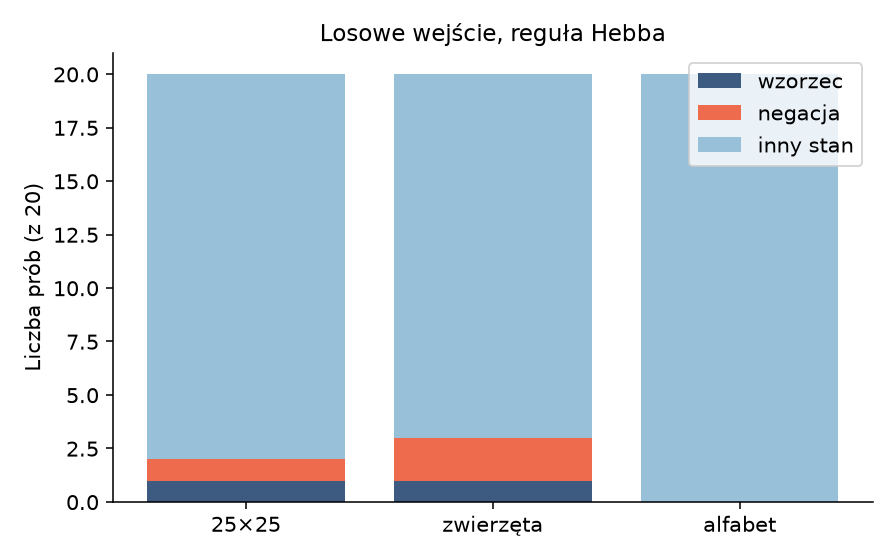
\includegraphics[width=0.72\textwidth]{losowe_wejscie.png}
    \caption{Klasyfikacja stanu końcowego po losowym starcie. Na alfabecie żaden przebieg nie kończy się literą.}
    \label{fig:random}
\end{figure}

\subsection{Opis wyników i dyskusja}
\begin{enumerate}
    \item \textbf{Losowy start rzadko trafia w nauczony rysunek.}
    Na \texttt{large-25x25} jedna próba z dwudziestu skończyła się dokładnym wzorcem, jedna jego negacją, a 18 innym stanem. Przestrzeń ma \(2^{625}\) punktów. Basen jednego z sześciu rysunków jest na tym tle mały. Część stanów pozornych leży tuż przy strzałce (595 zgodnych pikseli na 625), czyli przy jedynym wzorcu tego zbioru, który sam nie jest stabilny. Inne leżą przy szachownicy, ale tylko w około 320--340 pikselach na 625.

    \item \textbf{Negacja jest atraktorem, choć nie była uczona.}
    Na \(25\times 25\) pojawiła się jedna dokładna negacja, na zwierzętach dwie. Jeżeli \(s\) jest stabilny i pola są niezerowe, \(-s\) też jest stabilny, bo \(h(-s) = -h(s)\). Losowe wejście może więc wpaść w odwrócony rysunek.

    \item \textbf{Zwierzęta zbierają się w znanej mieszance.}
    Z 20 startów jeden trafił we wzorzec, dwa w negację, a 17 w inny stan. Te inne stany to głównie mieszanka z sekcji~\ref{sec:exp_stability} (około 106--107 zgodnych pikseli ze wzorcem 3) albo otoczenie jednego ze stabilnych zwierząt. Sieć nie błądzi równomiernie po wszystkich \(2^{126}\) stanach. Spada do kilku głębokich minimów.

    \item \textbf{Alfabet nie ma liter jako atraktorów.}
    Żadna z 20 prób nie kończy się literą ani jej negacją. Dwa stany pozorne powtarzają się wielokrotnie: jeden leży blisko litery 18 (270/280), drugi jest daleko od najbliższej litery (52/280). Brak stabilnych wzorców uczących nie oznacza braku minimów energii. Losowe wejście schodzi do tych minimów.
\end{enumerate}

\section{Eksperyment 6: Zbiór \(5\times 5\) o samych stabilnych wzorcach}
\label{sec:exp_5x5}

\subsection{Opis eksperymentu}
Zadanie każe zaproponować możliwie liczny zbiór wektorów o długości 25, taki żeby po uczeniu każdy wzorzec był stabilny. Losowa pojemność dałaby tu tylko około \(0{,}14 \cdot 25 \approx 3\) wzorce. Da się uzyskać więcej, jeżeli iloczyny skalarne są małe.

Dwa wektory \(\pm 1\) o nieparzystej długości nie mogą być prostopadłe: iloczyn \(N - 2d\) jest nieparzysty, więc najmniejszy moduł to 1. Szukano zbioru, w którym \(|x^{\mu}\cdot x^{\nu}| \le 1\) dla każdej pary. Z~\eqref{eq:field} wynika wtedy
\begin{equation}
    h_i x_i \ge 1 - \frac{P}{N} - \frac{P-1}{N} = \frac{N - 2P + 1}{N}.
\end{equation}
Dla \(N = 25\) prawa strona jest dodatnia przy \(P \le 12\) i nieujemna przy \(P = 13\). Taki zbiór jest więc stabilny co najmniej do trzynastu wzorców, a przy \(P = 13\) pole zerowe i tak zostawia bit bez zmiany.

Przeszukano układy z 12 albo 13 bitami ujemnymi, żądając kontrolowanego przecięcia nośników, dla dwunastu ziaren i \(150\,000\) prób na ziarno. Do najlepszego układu dołożono wektor samych jedynek. Ma on iloczyn \(\pm 1\) z każdym wektorem o 12 albo 13 bitach ujemnych. Zbiór nauczono regułą Hebba i sprawdzono stabilność każdego wzorca. Wzorce są na rysunku~\ref{fig:five}.

\begin{figure}[!htbp]
    \centering
    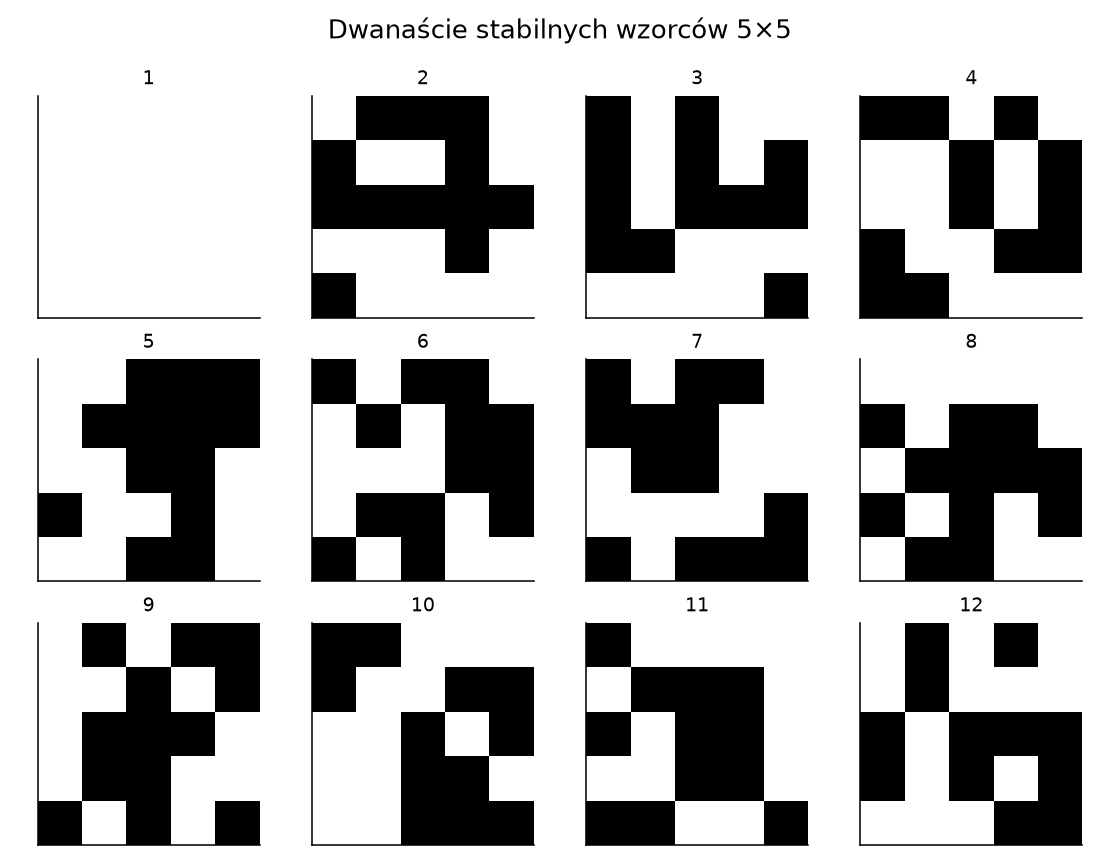
\includegraphics[width=0.72\textwidth]{zbior_5x5.png}
    \caption{Dwanaście wzorców \(5\times 5\). Po regule Hebba każdy jest stanem stabilnym. Największy moduł iloczynu dwóch różnych wzorców wynosi 1.}
    \label{fig:five}
\end{figure}

\subsection{Opis wyników i dyskusja}
\begin{enumerate}
    \item \textbf{Dwanaście wzorców, wszystkie stabilne.}
    Zbiór ma 12 wektorów. Po Hebba stabilne są wszystkie. Największy moduł iloczynu par wynosi 1. Zbiór jest zapisany w \texttt{experiments/results/stable-5x5.csv}. Wynik leży wewnątrz warunku wyprowadzonego z~\eqref{eq:field} i wyraźnie powyżej około trzech wzorców, których można oczekiwać przy losowym doborze.

    \item \textbf{Nie osiągnięto sufitu 13.}
    Wyszukiwanie nie znalazło trzynastego wektora spełniającego \(|x\cdot y| \le 1\) wobec wszystkich poprzednich. Sufit 13 jest warunkiem wystarczającym, a nie konstrukcją. Brak trzynastego wektora w próbie \(12 \times 150\,000\) nie obala oszacowania. Pokazuje tylko, że równomierne losowanie nośników słabo trafia w ostatni dopuszczalny wektor.
\end{enumerate}

\section{Eksperyment 7: Oscylacja między dwoma stanami}
\label{sec:exp_cycle}

\subsection{Opis eksperymentu}
Zadanie każe podać zbiór uczący i wzorzec wejściowy, po którym sieć krąży między dwoma stanami. Zbiór uczący składa się z jednego wzorca \(4\times 4\): białego kwadratu, czyli wektora samych jedynek. Wejście jest szachownicą. Przy jednym wzorcu złożonym z jedynek i przy parzystym \(N\) pole Hebba na stanie \(s\) redukuje się do
\begin{equation}
    h_i = \frac{1}{N}\sum_{j \neq i} s_j = \frac{1}{N}\Bigl(\sum_{j=1}^{N} s_j - s_i\Bigr).
\end{equation}
Suma bitów szachownicy wynosi zero, więc \(h_i = -s_i/N\). Znak pola jest przeciwny do stanu. Krok synchroniczny przełącza szachownicę na szachownicę przeciwną, a kolejny krok wraca do pierwszej.

Ten sam start puszczono asynchronicznie, z ziarnem 0. Oba przebiegi są na rysunku~\ref{fig:cycle}.

\begin{figure}[!htbp]
    \centering
    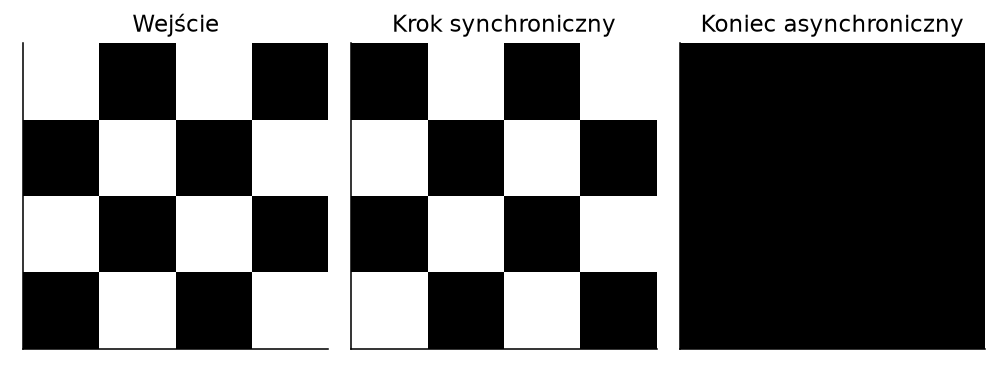
\includegraphics[width=0.92\textwidth]{oscylacja.png}
    \caption{Szachownica na wejściu, stan po jednym kroku synchronicznym oraz stan, do którego schodzi aktualizacja asynchroniczna. Kolejny krok synchroniczny wraca do lewej szachownicy.}
    \label{fig:cycle}
\end{figure}

\subsection{Opis wyników i dyskusja}
\begin{enumerate}
    \item \textbf{Synchronia krąży, energia stoi.}
    Status przebiegu synchronicznego to \texttt{cycle}, po dwóch krokach. Energia wynosi \(0{,}50 \to 0{,}50 \to 0{,}50\). Znak pola jest dokładnie przeciwny do stanu, więc sieć nie zbliża się do białego kwadratu. Przeskakuje między dwiema szachownicami. To jest możliwe tylko dlatego, że wszystkie neurony czytają ten sam stan. Wyprowadzenie \(\Delta E = -2|h_k|\) wymaga zmiany jednego neuronu przy pozostałych zamrożonych.

    \item \textbf{Asynchronia schodzi do negacji wzorca.}
    Po jednym pełnym przejściu energia spada z \(0{,}50\) do \(-7{,}50\), a stanem końcowym jest czarny kwadrat. Czarny kwadrat jest negacją wzorca uczącego, więc jest minimum energii. Przykład rozdziela dwie rzeczy pokazane przez Hopfielda \cite{hopfield1982}: spadek energii gwarantuje aktualizacja po jednym neuronie, a aktualizacja jednoczesna dopuszcza cykl o okresie dwa.
\end{enumerate}

\section{Eksperyment 8: Duże bitmapy}
\label{sec:exp_cats}

\subsection{Opis eksperymentu}
Duże bitmapy nie były dołączone do projektu. Pobrano trzy zdjęcia kotów z Wikimedia Commons: \texttt{Cat03.jpg}, \texttt{Kittyply\_edit1.jpg} i \texttt{Cat\_November\_2010-1a.jpg}. Każde zamieniono na obraz szary, przeskalowano do \(300 \times 200\) i sprogowano medianą jasności do wartości \(\pm 1\). Powstały trzy wzorce po \(N = 60\,000\) neuronów, czyli powyżej wymaganego minimum \(200 \times 300\).

Macierz \(60\,000 \times 60\,000\) nie była budowana. Pole liczono wzorem~\eqref{eq:implicit}. Sprawdzono stabilność każdego zdjęcia jednym krokiem synchronicznym, a następnie odwrócono 10\% pikseli pierwszego kota (\(6000\) bitów) i puszczono zbieganie.

\subsection{Wyniki eksperymentu}
Każde ze zdjęć jest stabilne: jeden krok zostawia wszystkie \(60\,000\) pikseli. Po uszkodzeniu sieć wraca do oryginału w jednym kroku, ze zgodnością 100\%. Przebieg jest na rysunku~\ref{fig:cats}.

\begin{figure}[!htbp]
    \centering
    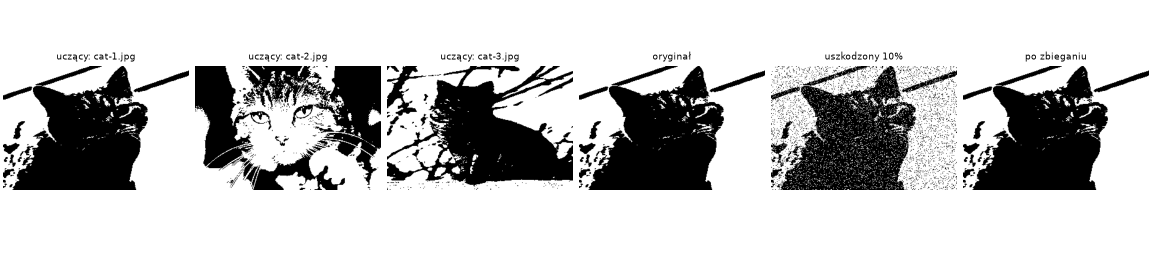
\includegraphics[width=\textwidth]{cats-recovery.png}
    \caption{Trzy wzorce uczące, oryginał pierwszego kota, ten sam obraz z 10\% odwróconych pikseli i stan po jednym kroku.}
    \label{fig:cats}
\end{figure}

\subsection{Opis wyników i dyskusja}
\begin{enumerate}
    \item \textbf{Małe \(P\) i różne obrazy zostawiają szeroki basen.}
    Przy \(P = 3\) sygnał w~\eqref{eq:field} wynosi \(1 - 3/60\,000\). Trzy fotografie po progowaniu medianą nie są swoimi kopiami, więc iloczyny skalarne nie są rzędu \(N\). Przesłuch nie przebija sygnału i jeden krok synchroniczny koryguje 10\% losowych błędów. To jest przeciwny biegun zbioru liter: tam \(P\) też nie było duże wobec \(N\), ale wzorce były prawie identyczne.

    \item \textbf{Wzór bez macierzy jest tym samym Hebbem.}
    Wyzerowanie przekątnej daje właśnie odejmowanie \((P/N)s\) we wzorze~\eqref{eq:implicit}. Sprawdzenie na małym zbiorze zwierząt daje ten sam następny stan co pełna macierz wag. Eksperyment nie zmienia reguły uczenia. Omija tylko zapis \(N^2\) liczb.
\end{enumerate}

\section{Podsumowanie i wnioski ogólne}
\label{sec:summary}

Zaimplementowano pamięć Hopfielda w \texttt{numpy}, z regułą Hebba, regułą Oji, dynamiką synchroniczną i asynchroniczną oraz z podglądem kolejnych stanów jako bitmapy. Liczba neuronów jest długością wzorca. Pomiary pozwalają sformułować następujące wnioski:

\begin{enumerate}
    \item \textbf{Dlaczego uczenie działa.}
    Reguła Hebba wpisuje do wagi współaktywność pikseli. Przy odtworzeniu własny wzorzec daje sygnał o znaku swojego bitu, a pozostałe wzorce dodają przesłuch. Reguła Oji robi ten sam krok i dokłada tłumienie, które utrzymuje wagi w ograniczeniu. Po zbieżności obie macierze różnią się dodatnią skalą, więc mają te same atraktory. Pomiar to potwierdza: liczby stabilnych wzorców są zgodne poza jednym, marginalnym znakiem OCRA.

    \item \textbf{Które zbiory są zapamiętane.}
    Poprawnie zapamiętany jest zbiór \(25\times 25\) (5 z 6). Częściowo zapamiętane są \(7\times 7\) (3 z 5), zwierzęta (2 z 6) i OCRA po Hebba (1 z 7). Nie są zapamiętane litery, alfabet ani rozciągnięty zbiór \(25\times 50\). We wszystkich tych przypadkach \(\alpha < 0{,}14\). Wzorce nie są stabilne, gdy iloczyny skalarne są duże wobec \(N\).

    \item \textbf{Odzysk i rodzaj zbioru.}
    Uszkodzony oryginał wraca tylko wtedy, gdy sam jest atraktorem, i tylko dopóki szum nie wyrzuci stanu z jego basenu. Przy \(P = 6\) i \(N = 625\) szóstka o średniej zgodności \(69\%\) nie utrwala żadnego wzorca, a szóstka o średniej zgodności \(51\%\) utrwala wszystkie i odzyskuje je także przy \(30\%\) szumu. Rozciągnięcie do \(25\times 50\) podnosi zgodność par do 74--87\% i zeruje odzysk, choć neuronów jest dwa razy więcej.

    \item \textbf{Losowe wejście, zbiór \(5\times 5\), oscylacja i koty.}
    Losowy start prawie nigdy nie trafia w nauczony rysunek. Ląduje w negacji albo w stanie pozornym. Przy iloczynach ograniczonych przez 1 da się utrwalić 12 wzorców o długości 25, wobec około trzech wzorców losowych. Szachownica na białym kwadracie \(4\times 4\) oscyluje synchronicznie przy stałej energii i schodzi asynchronicznie do czarnego kwadratu. Trzy zdjęcia kotów \(300\times 200\) są stabilne i korygują 10\% uszkodzeń w jednym kroku.
\end{enumerate}

\begin{thebibliography}{9}

\bibitem{hebb1949}
D.~O. Hebb.
\newblock \emph{The Organization of Behavior}.
\newblock Wiley, 1949.

\bibitem{hopfield1982}
J.~J. Hopfield.
\newblock Neural networks and physical systems with emergent collective computational abilities.
\newblock \emph{Proc. Natl. Acad. Sci. USA}, 79:2554--2558, 1982.

\bibitem{oja1982}
E.~Oja.
\newblock A simplified neuron model as a principal component analyzer.
\newblock \emph{J. Math. Biology}, 15:267--273, 1982.

\bibitem{amit1985}
D.~J. Amit, H.~Gutfreund, H.~Sompolinsky.
\newblock Spin-glass models of neural networks.
\newblock \emph{Phys. Rev. A}, 32:1007--1018, 1985.

\bibitem{amit1987}
D.~J. Amit, H.~Gutfreund, H.~Sompolinsky.
\newblock Statistical mechanics of neural networks near saturation.
\newblock \emph{Ann. Physics}, 173:30--67, 1987.

\bibitem{mceliece1987}
R.~J. McEliece, E.~C. Posner, E.~R. Rodemich, S.~S. Venkatesh.
\newblock The capacity of the Hopfield associative memory.
\newblock \emph{IEEE Trans. Inf. Theory}, 33:461--482, 1987.

\end{thebibliography}

\end{document}
